\documentclass[12pt,aspectratio=169]{beamer}
\setbeamertemplate{background}{%
 \includegraphics[width=\paperwidth]{BG/Background.pdf}
}
\usefonttheme{serif}
\input{Khaibao/KBChung}
\input{Khaibao/DeBai}
\linespread{1.2}
\begin{document}

\tieude{{\LARGE NGUYÊN HÀM}}

%\setcounter{section}{1}
\section{Nguyên hàm}

\subsection{Nguyên hàm của một hàm số}

%%%===============tomtat1==================
\begin{tomtat}
	\begin{dn}
		Cho hàm số $f(x)$ được xác định trên khoảng $K$ (hoặc một đoạn, hay một nửa khoảng). Hàm số $F(x)$ được gọi là một \textbf{nguyên hàm} của hàm số $f(x)$ trên $K$ nếu $F'(x) = f(x)$ với mọi $x$ thuộc~$K$.
	\end{dn}

	\begin{note}
		Trường hợp $K = [a;b]$ thì các đẳng thức $F'(a) = f(a)$ và $F'(b) = f(b)$ được hiểu là đạo hàm bên phải tại điểm $x = a$ và đạo hàm bên trái tại điểm $x = b$ của hàm số $F(x)$, tức là
		\[\lim\limits_{x\to a^{+}} \dfrac{F(x) - F(a)}{x - a} = f(a)\] và \[\lim\limits_{x\to b^{-}} \dfrac{F(x) - F(b)}{x - b} = f(b).\]
	\end{note}
\end{tomtat}

%%%===============vd1==================
\begin{vd}
	Cho hàm số $f(x) = x^2 - 2x$. Trong các hàm số đã cho dưới đây, hàm số nào là một nguyên hàm của $f(x)$ trên $\mathbb{R}$?
	\begin{enumEX}{2}
		\item $F(x) = \dfrac{x^3}{3} - x^2$;
		\item $G(x) = \dfrac{x^3}{3} + x^2$.
	\end{enumEX}

	\begin{loigiai}
		Ta có $F'(x) = x^2 - 2x$, $G'(x) = x^2 + 2x$.\\
		Vì $F'(x) = f(x)$ với mọi $x \in \mathbb{R}$ nên hàm số $F(x)$ là một nguyên hàm của hàm số $f(x)$ trên $\mathbb{R}$.\\
		Hàm số $G(x)$ không phải là một nguyên hàm của hàm số $f(x)$ trên $\mathbb{R}$ vì với $x = 1$, ta có
		\[G'(1) = 3 \neq -1 = f(1).\]
	\end{loigiai}
\end{vd}

%%%===============tomtat3==================
\begin{tomtat}
	\begin{dn}
		Giả sử $F(x)$ là một nguyên hàm của hàm số $f(x)$ trên $K$. Khi đó:
		\begin{enumerate}
			\item Với mỗi hằng số $C$, hàm số $F(x) + C$ cũng là một nguyên hàm của $f(x)$ trên $K$;
			\item Nếu hàm số $G(x)$ là một nguyên hàm của $f(x)$ trên $K$ thì tồn tại một hằng số $C$ sao cho $G(x) = F(x) + C$ với mọi $x \in K$.
		\end{enumerate}
		Như vậy, nếu $F(x)$ là một nguyên hàm của $f(x)$ trên $K$ thì mọi nguyên hàm của $f(x)$ trên $K$ đều có dạng $F(x) + C$ ($C$ là hằng số). Ta gọi $F(x) + C$ ($C \in \mathbb{R}$) là \textbf{họ các nguyên hàm} của $f(x)$ trên $K$, kí hiệu bởi $\displaystyle\int f(x)\mathrm{\,d}x$
	\end{dn}
\end{tomtat}
%%%===============tomtat4==================
\begin{tomtat}
	\begin{note}
		\begin{enumerate}[itemsep=6pt]
			\item Để tìm họ các nguyên hàm (gọi tắt là tìm nguyên hàm) của hàm số $f(x)$ trên $K$, ta chỉ cần tìm một nguyên hàm của $F(x)$ trên $f(x)$ trên $K$ và khi đó
			
			\medskip
			\begin{cangiua}
				$\displaystyle\int f(x)\mathrm{\,d}x = F(x) + C$, $C$ là hằng số.
			\end{cangiua}
			
			\item Người ta chứng minh được rằng, nếu hàm số $f(x)$ liên tục trên khoảng $K$ thì $f(x)$ có nguyên hàm trên khoảng đó.
			\item Biểu thức $f(x)\mathrm{\,d}x$ gọi là vi phân của nguyên hàm $F(x)$, kí hiệu là $\mathrm{\,d}F(x)$.\\
			Vậy $\mathrm{\,d}F(x) = F'(x)\mathrm{\,d}x = f(x)\mathrm{\,d}x$.
			\item Khi tìm nguyên hàm của một hàm số mà không chỉ rõ tập $K$, ta hiểu là tìm nguyên hàm của hàm số đó trên tập xác định của~nó.
		\end{enumerate}
	\end{note}
\end{tomtat}

%%%===============vd2==================
\begin{vd}\label{vd2}
	Tìm một nguyên hàm của hàm số $f(x) = x^2$ trên $\mathbb{R}$. từ đó hãy tìm $\displaystyle\int f(x)\mathrm{\,d}x$.

	\begin{loigiai}
		Vì $\left(\dfrac{x^3}{3}\right)'=\dfrac{3x^2}{3}=x^2$ nên $F(x)=\dfrac{x^3}{3}$ là một nguyên hàm của hàm số $f(x)$ trên $\mathbb{R}$.\\
		Do đó $\displaystyle\int x^2\mathrm{\,d}x=\dfrac{x^3}{3}+C$.
	\end{loigiai}
\end{vd}

\subsection{Tính chất cơ bản của nguyên hàm}

%%%===============tomtat5==================
\begin{tomtat}
	\begin{tc}
		Cho $f(x)$, $g(x)$ là hai hàm số liên tục trên $K$.
		\begin{itemize}
			\item $\displaystyle\int k f(x)\mathrm{\,d}x=k\displaystyle\int f(x)\mathrm{\,d}x$, với $k$ là hằng số khác $0$;
			\item $\displaystyle\int\left[f(x)+g(x)\right]\mathrm{\,d}x=\int f(x)\mathrm{\,d}x+\int g(x)\mathrm{\,d}x$;
			\item $\displaystyle \int\left[f(x)-g(x)\right]\mathrm{\,d}x=\int f(x)\mathrm{\,d}x-\int g(x)\mathrm{\,d}x$.
		\end{itemize}
	\end{tc}
\end{tomtat}

%%%===============vd3==================
\begin{vd}
	Sử dụng kết quả của Ví dụ \ref{vd2}, hãy tìm:
	\begin{enumEX}{2}
		\item $\displaystyle\int 3x^2\mathrm{\,d}x$;
		\item $\displaystyle\int -\dfrac{3}{2}x^2\mathrm{\,d}x$.
	\end{enumEX}

	\begin{loigiai}
		Ta có:
		\begin{enumerate}
			\item $\displaystyle\int 3x^2\mathrm{\,d}x = 3\displaystyle\int x^2\mathrm{\,d}x = 3\cdot\dfrac{x^3}{3}+C=x^3+C$.
			\item $\displaystyle\int -\dfrac{3}{2}x^2\mathrm{\,d}x = -\dfrac{3}{2}\displaystyle\int x^2\mathrm{\,d}x=-\dfrac{3}{2}\cdot\dfrac{x^3}{3}+C=-\dfrac{1}{2}x^3+C$.
		\end{enumerate}
	\end{loigiai}
\end{vd}

%%%===============vd4==================
\begin{vd}
	Sử dụng tính chất cơ bản của nguyên hàm, hãy tìm:
	\begin{enumEX}{2}
		\item $\displaystyle\int \left(x^2+x\right)\mathrm{\,d}x$;
		\item $\displaystyle\int \left(4x^3-3x^2\right)\mathrm{\,d}x$.
	\end{enumEX}

	\begin{loigiai}
		Ta có:
		\begin{enumerate}
			\item $\displaystyle\int \left(x^2+x\right)\mathrm{\,d}x = \displaystyle\int x^2\mathrm{\,d}x + \displaystyle\int x\mathrm{\,d}x = \dfrac{x^3}{3} + \dfrac{x^2}{2} + C$.
			\item $\displaystyle\int \left(4x^3-3x^2\right)\mathrm{\,d}x = 4\displaystyle\int x^3\mathrm{\,d}x - 3\displaystyle\int x^2 \mathrm{\,d}x = x^4-x^3 + C$.
		\end{enumerate}
	\end{loigiai}
\end{vd}

\begin{frame}[allowframebreaks]
\noindent
{\color{mauvang}\textbf{Vận dụng.}} Doanh thu bán hàng của một công ty khi bán một loại sản phẩm là số tiền $R(x)$ (triệu đồng) thu được khi $x$ đơn vị sản phẩm được bán ra. Tốc độ biến động (thay đổi) của doanh thu khi $x$ đơn vị sản phẩm đã được bán là hàm số $M_R(x)=R'(x)$. Một công ty công nghệ cho biết, tốc độ biến đổi của doanh thu khi bán một loại con chíp của hãng được cho bởi $M_R(x) = 300 – 0{,}1x$, ở đó $x$ là số lượng chíp đã bán. Tìm doanh thu của công ty khi đã bán $1 000$ con chíp.

\textit{Hướng dẫn:} Vì $R'(x) = M_R(x)$ nên doanh thu $R(x)$ là một nguyên hàm của $M_R(x)$.

\noindent
\textbf{Lời giải}.
	Theo giả thiết, ta có $M_R(x)=R'(x)$ nên $R(x)$ là một nguyên hàm của hàm số $M_R(x)$. Do đó
	$$R(x)=\displaystyle M_R(x) \mathrm{\, d}x=300x-\dfrac{1}{20}x^2+C.$$
	Vì Doanh thu bán hàng của công ty đó là $R(x)$ thu được khi bán được $x$ đơn vị sản phẩm nên $R(0)=0\Leftrightarrow C=0\Rightarrow R(x)=300x-\dfrac{1}{20}x^2$.\\
	Vậy doanh thu của công ty khi đã bán $1000$ con chíp là
	$$R(1000)=300\cdot 1000 - \dfrac{1}{20}\cdot 1000 = 299950 \text{ (triệu đồng)}.$$
\end{frame}

\subsection{Nguyên hàm của một số hàm số thường gặp}

%%%===============tomtat6==================
\begin{tomtat}
	\begin{dl}
		\begin{multicols}{2}
			\begin{itemize}
				\item Với $\alpha\ne -1$, ta có \\
				$\displaystyle\int x^{\alpha}\mathrm{\,d}x=\dfrac{x^{\alpha+1}}{\alpha+1}+C$;
				\item $\displaystyle \int\dfrac{1}{x}\mathrm{\,d}x=\ln|x|+C$;
				\item $\displaystyle \int\cos x\mathrm{\,d}x=\sin x+C$;
				\item $\displaystyle \int \sin x\mathrm{\,d}x=-\cos x+C$;
				\item $\displaystyle \int \dfrac{1}{\cos^2x}\mathrm{\,d}x=\tan x+C$;
				\item $\displaystyle \int \dfrac{1}{\sin^2x}\mathrm{\,d}x=-\cot x+C$;
				\item $\displaystyle\int\mathrm{e}^x\mathrm{\,d}x=\mathrm{e}^x+C$;
				\item $\displaystyle\int a^x\mathrm{\,d}x=\dfrac{a^x}{\ln a}+C$\\ ($a>0$, $a\ne 1$).
			\end{itemize}
		\end{multicols}
	\end{dl}
\end{tomtat}

%%%===============vd5==================
\begin{vd}
	Tìm:
	\begin{enumEX}{3}
		\item $\displaystyle\int \sqrt{x}\mathrm{\,d}x$ ($x>0$);
		\item $\displaystyle\int \dfrac{1}{x^3}\mathrm{\,d}x$;
		\item $\displaystyle\int \left(2x^2+\dfrac{3}{\sqrt{x}}\right)\mathrm{\,d}x$.
	\end{enumEX}

	\begin{loigiai}
		\begin{enumerate}
			\item $\displaystyle\int \sqrt{x}\mathrm{\,d}x = \displaystyle\int x^{\tfrac{1}{2}}\mathrm{\,d}x = \dfrac{x^{\tfrac{1}{2}+1}}{\frac{1}{2}+1} + C = \dfrac{2}{3}x^{\tfrac{3}{2}} + C = \dfrac{2}{3}x\sqrt{x}+C$.
			\item $\displaystyle\int \dfrac{1}{x^3}\mathrm{\,d}x = \displaystyle\int x^{-3}\mathrm{\,d}x = \dfrac{x^{-3+1}}{-3+1} + C = -\dfrac{1}{2}x^{-2} + C = -\dfrac{1}{2x^2}+C$.
			\item $\displaystyle\int \left(2x^2+\dfrac{3}{\sqrt{x}}\right)\mathrm{\,d}x = \displaystyle\int 2x^2\mathrm{\,d}x + \displaystyle\int \dfrac{3}{\sqrt{x}}\mathrm{\,d}x = 2\displaystyle\int x^2\mathrm{\,d}x + 3\displaystyle\int \dfrac{1}{\sqrt{x}} \mathrm{\,d}x = 2x^3 + 6\sqrt{x} + C$.
		\end{enumerate}
	\end{loigiai}
\end{vd}

\subsubsection{Nguyên hàm của hàm số lượng giác}

%%%===============tomtat7==================
\begin{tomtat}
	\begin{dl}
		\begin{itemize}
			\item $\displaystyle\int \cos x\mathrm{\,d}x = \sin x + C$;
			\item $\displaystyle\int \sin x\mathrm{\,d}x = -\cos x + C$;
			\item $\displaystyle\int \dfrac{1}{\cos^2 x}\mathrm{\,d}x = \tan x + C$;
			\item $\displaystyle\int \dfrac{1}{\sin^2 x}\mathrm{\,d}x = \cot x + C$.
		\end{itemize}
	\end{dl}
\end{tomtat}

%%%===============vd6==================
\begin{vd}
	Tìm:
	\begin{enumerate}
		\item $\displaystyle\int (\cos x + \sin x)\mathrm{\,d}x$;
		\item $\displaystyle\int\left(2\cos x + \dfrac{1}{\cos^2 x}\right)\mathrm{\,d}x$.
	\end{enumerate}

	\begin{loigiai}
		\begin{enumerate}
			\item $\displaystyle\int (\cos x + \sin x)\mathrm{\,d}x = \displaystyle\int \cos x\mathrm{\,d}x + \displaystyle\int \sin x\mathrm{\,d}x = \sin x - \cos x + C$;
			\item $\displaystyle\int (2\cos x + \dfrac{1}{\cos^2 x})\mathrm{\,d}x = 2\displaystyle\int \cos x\mathrm{\,d}x - \displaystyle\int \dfrac{1}{\cos^2 x}\mathrm{\,d}x = 2\sin x - \tan x + C$.
		\end{enumerate}
	\end{loigiai}
\end{vd}

\subsubsection{Nguyên hàm của hàm số mũ}

%%%===============tomtat8==================
\begin{tomtat}
	\begin{dl}
		\begin{itemize}
			\item $\displaystyle\int \mathrm{e}^x\mathrm{\,d}x = \mathrm{e}^x + C$;
			\item $\displaystyle\int a^x\mathrm{\,d}x = \dfrac{a^x}{\ln a} + C$ ($0<a\neq1$).
		\end{itemize}
	\end{dl}
\end{tomtat}

%%%===============vd7==================
\begin{vd}
	Tìm:
	\begin{enumEX}{3}
		\item $\displaystyle\int 2^x\mathrm{\,d}x$;
		\item $\displaystyle\int \dfrac{1}{3^x}\mathrm{\,d}x$;
		\item $\displaystyle\int \left(2\mathrm{e}^x-5^x\right)\mathrm{\,d}x$.
	\end{enumEX}

	\begin{loigiai}
		\begin{enumerate}
			\item $\displaystyle\int 2^x\mathrm{\,d}x = \dfrac{2^x}{\ln 2} + C$;
			\item $\displaystyle\int \dfrac{1}{3^x}\mathrm{\,d}x = \displaystyle\int \left(\dfrac{1}{3}\right)^x\mathrm{\,d}x = \dfrac{\left(\dfrac{1}{3}\right)^x}{\ln\dfrac{1}{3}} + C = -\dfrac{1}{3^x \ln 3} + C$;
			\item $\displaystyle\int \left(2\mathrm{e}^x-5^x\right)\mathrm{\,d}x = 2 \displaystyle\int \mathrm{e}^x\mathrm{\,d}x - \displaystyle\int 5^x\mathrm{\,d}x = 2\mathrm{e}^x - \dfrac{5^x}{\ln 5} + C$.
		\end{enumerate}
	\end{loigiai}
\end{vd}

\begin{tomtat}
Ta tổng kết lại nguyên hàm của một số hàm số thường gặp như sau
%\renewcommand{\arraystretch}{1.8}
\begin{center}
\renewcommand{\arraystretch}{1.5}
	\begin{tabular}{|l|l|} \hline
		$\displaystyle\int 0 \mathrm{\,d}x = C$& $\displaystyle\int 1\mathrm{\,d}x = x + C$\\ \hline
		$\displaystyle\int x^\alpha\mathrm{\,d}x = \dfrac{x^{\alpha+1}}{\alpha + 1} + C$ ($\alpha\neq-1)$& $\displaystyle\int \dfrac{1}{x}\mathrm{\,d}x = \ln|x| + C$\\ \hline
		$\displaystyle\int \mathrm{e}^x\mathrm{\,d}x = \mathrm{e}^x + C$& $\displaystyle\int a^x\mathrm{\,d}x = \dfrac{a^x}{\ln a} + C$ ($0<a\neq1$)\\ \hline
		$\displaystyle\int \cos x\mathrm{\,d}x = \sin x + C$& $\displaystyle\int \sin x\mathrm{\,d}x = -\cos x + C$\\ \hline
		$\displaystyle\int \dfrac{1}{\sin^2 x}\mathrm{\,d}x = -\cot x + C$& $\displaystyle\int \dfrac{1}{\cos^2 x}\mathrm{\,d}x = \tan x + C$\\ \hline
	\end{tabular}
\end{center}
\end{tomtat}

\subsection{Trắc nghiệm một phương án đúng}
%Học sinh trả lời từ câu 1 đến câu 12. Mỗi câu học sinh chỉ chọn một phương án.

%%%===============tracnghiem1==================
\begin{tracnghiem}%[2D4N1-1]
	Phát biểu nào sau đây là đúng?

	\choice
		{\True $\displaystyle\int F'(x) \mathrm{\,d} x=F(x)+C$}
		{$\displaystyle\int F(x) \mathrm{\,d} x=F'(x)+C$}
		{$\displaystyle\int F(x) \mathrm{\,d} x=F(x)+C$}
		{$\displaystyle\int F'(x) \mathrm{\,d} x=F'(x)+C$}

	\begin{loigiai}
			Ta có $\displaystyle\int F'(x) \mathrm{\,d} x=F(x)+C$.
	\end{loigiai}
\end{tracnghiem}

%%%===============tracnghiem2==================
\begin{tracnghiem}%[2D4N1-1]
	Cho hàm số $f(x)$ có đạo hàm là hàm liên tục trên $\mathbb{R}$. Phát biểu nào sau đây là đúng?

	\choice
		{$\displaystyle\int f(x) \mathrm{\,d}x=f'(x)+C$}
		{$\displaystyle\int f'(x) \mathrm{\,d}x=f(x)$}
		{$\displaystyle\int f(x) \mathrm{\,d}x=f'(x)$}
		{\True $\displaystyle\int f'(x) \mathrm{\,d}x=f(x)+C$}

	\begin{loigiai}
			Ta có $\displaystyle\int f'(x) \mathrm{\,d}x=f(x)+C$.
	\end{loigiai}
\end{tracnghiem}

%%%===============tracnghiem3==================
\begin{tracnghiem}%[2D4N1-1]
	Hàm số $F(x)$ là một nguyên hàm của hàm số $f(x)$ trên khoảng $K$ nếu

	\choice
		{$F'(x)=-f(x)$, $\forall x \in K$}
		{\True $F'(x)=f(x)$, $\forall x \in K$}
		{$f'(x)=F(x)$, $\forall x \in K$}
		{$f'(x)=-F(x)$, $\forall x \in K$}

	\begin{loigiai}
			Theo định nghĩa thì hàm số $F(x)$ là một nguyên hàm của hàm số $f(x)$ trên khoảng $K$ nếu $F'(x)=f(x)$,$\forall x \in K$.
	\end{loigiai}
\end{tracnghiem}

%%%===============tracnghiem4==================
\begin{tracnghiem}%[2D4N1-4]
	Một nguyên hàm của hàm số $f(x)=2\,025^x$ là

	\choice
		{$F(x)=x \cdot 2\,025^{x-1}$}
		{$F(x)=2\,025 \cdot 2\,024^x$}
		{$F(x)=2\,025^x \cdot \ln 2\,025$}
		{\True $F(x)=\dfrac{2\,025^x}{\ln 2\,025}$}

	\begin{loigiai}
			Ta có
			\[\displaystyle\int f(x)\mathrm{\,d}x=\displaystyle\int 2\,025^x\mathrm{\,d}x=\dfrac{2\,025^x}{\ln 2\,025}+C.\]
	\end{loigiai}
\end{tracnghiem}

%%%===============tracnghiem5==================
\begin{tracnghiem}%[2D4N1-2]
	Cho hàm số $y = f(x)$ là một nguyên hàm của hàm số $y = x^3$. Phát biểu nào sau đây là đúng?

	\choice
		{$f(x) = \dfrac{x^4}
		{4} + C$}
		{$f(x) = 3x^2$}
		{$f(x) = 4x^3$}
		{\True $f(x) = \dfrac{x^4}{4}$}

	\begin{loigiai}
			Hàm số $f(x) = \dfrac{x^4}{4}$ là một nguyên hàm của hàm số $y = x^3$ vì $f'(x) = x^3$.
	\end{loigiai}
\end{tracnghiem}

%%%===============tracnghiem6==================
\begin{tracnghiem}%[2D4N1-2]
	Hàm số nào sau đây là một nguyên hàm của hàm số $f(x)=\sin x$?

	\choice
		{$F_1(x)=\sin x$}
		{$F_2(x)=-\sin x$}
		{$F_3(x)=\cos x$}
		{\True $F_4(x)=-\cos x$}

	\begin{loigiai}
			Ta có $F(x)=\displaystyle\int f(x)\mathrm{\,d}x = \displaystyle\int \sin x\mathrm{\,d}x =-\cos x+C$ là họ nguyên hàm của hàm số $f(x)$.\\
			Nên $F(x)=-\cos x$ là một nguyên hàm của hàm số $f(x)=\sin x$.
	\end{loigiai}
\end{tracnghiem}

%%%===============tracnghiem7==================
\begin{tracnghiem}%[2D4H1-6]
	Giả sử một chất điểm chuyển động với gia tốc tại thời điểm $t$ (giây) được xác định bởi công thức $a(t)=2t-1$ (m/s$^2$). Biết rằng vận tốc của chất điểm tại thời điểm ban đầu là $v_0=2$ (m/s). Vận tốc của chất điểm đó tại thời điểm $t$ (giây) là

	\choice
		{$v(t)=2t^2-t+2$ m/s}
		{\True $v(t)=t^2-t+2$ m/s}
		{$v(t)=2t^2-t$ m/s}
		{$v(t)=t^2-t$ m/s}

	\begin{loigiai}
			Ta có $v(t)=\displaystyle\int (2t-1) \mathrm{\,d}t=t^2-t+C$.\\
			Ứng với $v_0=2$ thì $t=0$, khi đó ta có $C=2$.\\
			Vậy $v(t)=t^2-t+2$ m/s.
	\end{loigiai}
\end{tracnghiem}

%%%===============tracnghiem8==================
\begin{tracnghiem}%[2D4H1-2]
	Nguyên hàm của hàm số $f(x)=\dfrac{2\sqrt{x}-1}{x}$ trên khoảng $(0;+\infty)$ là

	\choice
		{$2\sqrt{x}+\ln x+C$}
		{$2\sqrt{x}-\ln x+C$}
		{$4\sqrt{x}+\ln x+C$}
		{\True $4\sqrt{x}-\ln x+C$}

	\begin{loigiai}
			Ta có $\displaystyle\int \dfrac{2\sqrt{x}-1}{x} \mathrm{\,d}x=\displaystyle\int \left(\dfrac{2}{\sqrt{x}}-\dfrac{1}{x}\right) \mathrm{\,d}x=4\sqrt{x}-\ln x+C$.
	\end{loigiai}
\end{tracnghiem}

%%%===============tracnghiem9==================
\begin{tracnghiem}%[2D4H1-2]
	Nguyên hàm của hàm số $f(x)=\dfrac{x-1}{x}$ là

	\choice
		{$x+\ln|x|+C$}
		{\True $x-\ln|x|+C$}
		{$x+\ln x+C$}
		{$x-\ln x+C$}

	\begin{loigiai}
			Ta có $\displaystyle\int f(x) \mathrm{\,d}x=\int\dfrac{x-1}{x} \mathrm{\,d}x=\int\left(1-\dfrac{1}{x}\right)\mathrm{d}x=x-\ln|x|+C$.
	\end{loigiai}
\end{tracnghiem}

%%%===============tracnghiem10==================
\begin{tracnghiem}%[2D4H1-4]
	Trong các hàm số dưới đây, hàm số nào có họ tất cả các nguyên hàm là $F(x)=\dfrac{a^x}{\ln a}+C$ với $a>0$, $a\ne 1$?

	\choice
		{\True $f(x)=a^x$}
		{$f(x)=\dfrac{1}
		{x}$}
		{$f(x)=\ln x$}
		{$f(x)=x^a$}

	\begin{loigiai}
			Ta có \[\displaystyle\int a^x\mathrm{\,d}x=\dfrac{a^x}{\ln a}+C.\]
	\end{loigiai}
\end{tracnghiem}

%%%===============tracnghiem11==================
\begin{tracnghiem}%[2D4H1-4]
	Cho hàm số $f(x)$ thoả mãn $f'(x)=2x-3\mathrm{e}^x$, $\forall x \in \mathbb{R}$ và $f(0)=5$. Khẳng định nào sau đây đúng?

	\choice
		{$f(x)=2x+3\mathrm{e}^x+2$}
		{$f(x)=x^2+3\mathrm{e}^x+2$}
		{$f(x)=2x-3\mathrm{e}^x+8$}
		{\True $f(x)=x^2-3\mathrm{e}^x+8$}

	\begin{loigiai}
			Ta có $f(x)=\displaystyle\int \left(2x-3\mathrm{e}^x\right) \mathrm{\,d}x=x^2-3\mathrm{e}^x+C$.\\
			Có $f(0)=5\Rightarrow C=8$. \\
			Vậy $f(x)=x^2-3\mathrm{e}^x+8$.
	\end{loigiai}
\end{tracnghiem}

%%%===============tracnghiem12==================
\begin{tracnghiem}%[2D4H1-3]
	$\displaystyle \int \left(\sin \dfrac{x}{2}+\cos\dfrac{x}{2} \right)^2 \mathrm{d}x$ bằng

	\choice
		{\True $x-\cos x+C$}
		{$\left(-\cos \dfrac{x}
		{2}+\sin\dfrac{x}
		{2} \right)^2$}
		{$\dfrac{1}{3} \left(\sin \dfrac{x}{2}+\cos\dfrac{x}{2}\right)^3+C$}
		{$x+\cos x+C$}

	\begin{loigiai}
			Ta có
			\allowdisplaybreaks
			\begin{eqnarray*}
				\displaystyle \int \left(\sin \dfrac{x}{2}+\cos\dfrac{x}{2} \right)^2 \mathrm{\,d}x &=& \displaystyle \int \left(\sin^2 \dfrac{x}{2}+\cos^2\dfrac{x}{2}+2\sin \dfrac{x}{2}\cos \dfrac{x}{2} \right) \mathrm{\,d}x\\
				&=& \displaystyle \int (1+\sin x) \mathrm{\,d}x\\
				&=& \displaystyle \int \mathrm{\,d}x+\displaystyle \int \sin x \mathrm{\,d}x\\
				&=& x-\cos x+C.
		\end{eqnarray*}
	\end{loigiai}
\end{tracnghiem}

\subsection{Dạng đúng sai}

%%%===============dungsai1==================
\begin{dungsai}%[2D4H1-3]
	Cho $F(x)=\displaystyle \int \tan^2x\mathrm{\,d}x$ và thỏa mãn $F(0)=0$. Khi đó

	\choiceTF
		{\True $F(x)=-x+\tan x$}
		{Hàm số $F(x)$ là hàm số chẵn trên tập xác định của $F(x)$}
		{\True Hàm số $F(x)$ đồng biến trên mỗi khoảng xác định của nó}
		{\True Phương trình $F(x)+x=0$ có các nghiệm là $x=k\pi$, $k\in \mathbb{Z}$}

	\begin{loigiai}
			\begin{itemchoice}
				\itemch Ta có
				\[\displaystyle F(x)=\int \tan^2x\mathrm{\,d}x
				=\int \left(\dfrac{1}{\cos^2x}-1\right)\mathrm{\,d}x
				=\tan x-x+C.\]
				Mặt khác $F(0)=0$ nên ta có $C=0$ nên $F(x)=-x+\tan x$.
				\itemch Ta thấy rằng $F(-x)=x-\tan x=-F(x)$ nên hàm số đã cho là hàm lẻ trên mỗi khoảng xác định của $F(x)$.
				\itemch Ta có $F'(x)=\tan^2x\ge 0$ với mọi $x$ thuộc tập xác định của $F(x)$ nên hàm số $F(x)$ đồng biến trên mỗi khoảng xác định của nó.
				\itemch Ta có
				\[F(x)+x=0\Leftrightarrow -x+\tan x+x=0\Leftrightarrow \tan x=0\Leftrightarrow x=k\pi,\,k\in \mathbb{Z}.\]
		\end{itemchoice}
	\end{loigiai}
\end{dungsai}

%%%===============dungsai2==================
\begin{dungsai}[n]%[2D4H1-2]
	Cho hàm số $f(x)=-3x^2+6x$ với tập xác định $\mathbb{R}$. Gọi $F(x)$ là nguyên hàm của hàm số $f(x)$ trên $\mathbb{R}$. Khi đó

	\choiceTF
		{\True $f(x)$ là một nguyên hàm của hàm số $g(x)=-6x+6$ trên $\mathbb{R}$}
		{\True $F(x)=-x^3+3x^2+C$ với $C$ là hằng số}
		{Nếu $F(0)=1$ thì $F(1)$ bằng $2$}
		{\True Nếu $F(1)=2$ thì $F(2\,024) > F(2\,025)$}

	\begin{loigiai}
			\begin{itemchoice}
				\itemch
				Ta có $f'(x)=-6x+6=g(x)$ nên $f(x)$ là một nguyên hàm của hàm số $g(x)$.
				\itemch Ta có $F(x)=\displaystyle\int f(x) \mathrm{\,d}x=\displaystyle\int (-3x^2+6x) \mathrm{\,d}x=-x^3+3x^2+C$.
				\itemch $F(0)=1\Rightarrow C=1$ nên $F(x)=-x^3+3x^2+1$.\\
				Khi đó $F(1)=-1+3+1=3$.
				\itemch
				$F(1)=2\Rightarrow 2+C=1\Leftrightarrow C=-1$ nên $F(x)=-x^3+3x^2-1$.\\
				Ta có $F'(x)=-3x^2+6x$.\\
				$F'(x)=0\Leftrightarrow \hoac {&x=0\\&x=2.}$\\
				Ta có bảng biến thiên
				\begin{center}
					
\begin{tikzpicture}
						\tkzTabInit[nocadre=false,lgt=1.5,espcl=2.5,deltacl=0.6]{$x$/0.7,$F'(x)$/0.7,$F (x)$/1.5}{$-\infty$,$0$,$2$,$+\infty$}
						\tkzTabLine{,-,0,+,0,-,}
						\tkzTabVar{+/$+\infty$,-/$ $,+/$ $,-/$-\infty$}
					\end{tikzpicture}
			\end{center}
			Theo bảng biến thiên, $F(x)$ nghịch biến trên $(2;+\infty)$ nên $F(2\,024) > F(2\,025)$.
		\end{itemchoice}
	\end{loigiai}
\end{dungsai}

%%%===============dungsai3==================
\begin{dungsai}[n]%[2D4V1-6]
	Một bể bơi hình trụ có đường kính $5$ m và chiều cao $1$ m; bể được bơm nước vào với tốc độ không đổi $v_0$. Sau khi nước được bơm đầy, bể bơi bị thủng một lỗ ở đáy và nước chảy ra ngoài; bể bơi chảy hết nước trong $8$ giờ. Biết tốc độ giảm chiều cao của bể bơi khi nước chảy ra ngoài vào thời điểm $t$ giờ (tính từ lúc nước đầy bể và ngừng bơm) được cho bởi hàm số $h'(t)=at+b$, với $a,b\in \mathbb{R}$. Lúc nước chảy hết ra ngoài thì tốc độ giảm chiều cao bằng $0$. Khi đó

	\choiceTF
		{Thể tích của bể bơi sau khi nước được làm đầy là $6{,}25\pi$ m$^3$}
		{$32a+1=0$ và $4b+1=0$}
		{Sau $4$ giờ kể từ lúc bể bị rò, lượng nước bị mất đi bằng $\dfrac{75\pi }{16}$ m$^3$}
		{Lượng nước bị rò rỉ ra ngoài một nửa sau $\left(8-4\sqrt{2}\right)$ giờ}

	\begin{loigiai}
			\begin{itemchoice}
				\itemch Bể nước hình trụ có bán kính đáy $r = 2{,}5$ m, chiều cao $h = 1$ m.\\
				Thể tích khi đầy $V = \pi r^2 h = \pi \cdot (2{,}5)^2 \cdot 1 = 6{,}25\pi$ m$^3$.
				\itemch Ta có $h'(8) = 0 \Rightarrow 8a + b = 0$. \quad (1)\\
				Chiều cao của nước thời điểm $t$ là $h(t) = \displaystyle\int (at+b)\mathrm{d}t = \dfrac{a}{2}t^2 + bt + c$.\\
				Vì $\heva{& h(0) = 1 \\ & h(8) = 0} \Rightarrow \heva{& c = 1 \\ & 32a + 8b + 1 = 0.}$ \quad (2)\\
				Từ (1) và (2) suy ra $a = \dfrac{1}{32}$, $b = -\dfrac{1}{4}$.\\ Khi đó $32a - 1 = 0$; $4b + 1 = 0$ và $h(t) = \dfrac{1}{64}t^2 - \dfrac{1}{4}t + 1$.
				\itemch Chiều cao mực nước trong bể sau $4$ giờ là $h(4) = \dfrac{1}{64} \cdot 4^2 - \dfrac{1}{4} \cdot 4 + 1 = 0{,}25$ m.\\
				Lượng nước còn lại trong bể sau $4$ giờ là $\pi r^2 \cdot h(4) = \pi \cdot (2{,}5)^2 \cdot 0{,}25 = \dfrac{25\pi}{16}$ m$^3$.\\
				Lượng nước đã thoát ra sau $4$ giờ là $6{,}25\pi - \dfrac{25\pi}{16} = \dfrac{75\pi}{16}$ m$^3$.
				\itemch Lượng nước còn lại khi đã mất một nửa là $\dfrac{6{,}25\pi}{2} = \dfrac{25\pi}{8}$ m$^3$.\\
				Chiều cao tương ứng $h(t_1)$ của bể thỏa mãn $\pi \cdot (2{,}5)^2 \cdot h(t_1) = \dfrac{25\pi}{8} \Rightarrow h(t_1) = 0{,}5$ m.\\
				Ta có $h(t_1) = \dfrac{1}{64}t_1^2 - \dfrac{1}{4}t_1 + 1 = 0{,}5 \Rightarrow \heva{&t_1 = 8 + 4\sqrt{2} \approx 13{,}7 > 8 \\ &t_1 = 8 - 4\sqrt{2} \approx 2{,}3 \in (0; 8).
				}$\\
				Ta thấy $t_1 = 8 - 4\sqrt{2}$ (giờ) thỏa mãn đề bài.
		\end{itemchoice}
	\end{loigiai}
\end{dungsai}

%%%===============dungsai4==================
\begin{dungsai}[n]%[2D4V1-6]
	\immini{
	Cây cà chua khi trồng có chiều cao $5$\,cm. Tốc độ tăng chiều cao của cây cà chua sau khi trồng được cho bởi hàm số $v(t)=-0{,}1t^3+t^2$, trong đó $t$ tính theo tuần, $v(t)$ tính bằng cm/tuần. Gọi $h(t)$ (tính bằng cm) là độ cao của cây cà chua ở tuần thứ $t$.	({\it Nguồn: A. Bigalke et al., Grundkurs ma-1, Cornelsen 2016}). Khi đó
	}{
	\resizebox{!}{3cm}{
	
\begin{tikzpicture}
		\definecolor{c628a12}{RGB}{98,138,18}
		\definecolor{ceb0000}{RGB}{235,0,0}
		\definecolor{cff3b3b}{RGB}{255,59,59}
		\definecolor{cff6666}{RGB}{255,102,102}
		\definecolor{c99cc33}{RGB}{153,204,51}
		\definecolor{c81b31e}{RGB}{129,179,30}
		\newcommand{\quacachua}{\tikz{
		\path[fill=c628a12,even odd rule] (0,0).. controls (-0.04,0.44) and (0,0.74).. (0.12,0.92).. controls (0.26,1.09) and (0.47,1.13).. (0.77,1.02) -- (0.75,0.95).. controls (0.48,1.05) and (0.3,1.02).. (0.19,0.87).. controls (0.07,0.72) and (0.03,0.43).. (0.07,0.01) -- cycle;
		\path[fill=c628a12,even odd rule] (-0.03,0.02).. controls (-0.33,0.02) and (-0.5,0.12).. (-0.65,0.23).. controls (-0.45,0.14) and (-0.25,0.09).. (-0.03,0.15).. controls (-0.19,0.28) and (-0.22,0.45).. (-0.22,0.64).. controls (-0.16,0.38) and (-0.01,0.21).. (0.12,0.14).. controls (0.35,0.05) and (0.57,0.09).. (0.78,0.16).. controls (0.56,0.03) and (0.33,-0.09).. (-0.03,0.02);
		\path[fill=ceb0000,even odd rule] (-0.03,0.09).. controls (0.38,0.09) and (0.7,-0.07).. (0.7,-0.47).. controls (0.7,-0.88) and (0.38,-1.2).. (-0.03,-1.2).. controls (-0.43,-1.2) and (-0.76,-0.88).. (-0.76,-0.47).. controls (-0.76,-0.07) and (-0.43,0.09).. (-0.03,0.09);
			}}
		\newcommand{\lacachua}{\tikz{
		\path[fill=c99cc33,even odd rule] (0,0).. controls (0.02,0.11) and (0.02,0.21).. (-0.01,0.3).. controls (-0.02,0.28) and (-0.04,0.27).. (-0.07,0.27).. controls (-0.08,0.35) and (-0.09,0.43).. (-0.11,0.5).. controls (-0.13,0.46) and (-0.15,0.42).. (-0.19,0.39).. controls (-0.22,0.5) and (-0.26,0.6).. (-0.35,0.68).. controls (-0.35,0.65) and (-0.35,0.62).. (-0.36,0.59).. controls (-0.4,0.66) and (-0.44,0.74).. (-0.51,0.78).. controls (-0.51,0.76) and (-0.51,0.73).. (-0.53,0.71).. controls (-0.59,0.78) and (-0.66,0.84).. (-0.77,0.86).. controls (-0.75,0.84) and (-0.73,0.82).. (-0.74,0.79).. controls (-0.82,0.82) and (-0.91,0.84).. (-1.01,0.84).. controls (-0.96,0.82) and (-0.91,0.79).. (-0.87,0.75).. controls (-0.9,0.74) and (-0.93,0.72).. (-0.96,0.71).. controls (-0.89,0.69) and (-0.84,0.65).. (-0.8,0.6).. controls (-0.84,0.6) and (-0.88,0.59).. (-0.91,0.57).. controls (-0.84,0.57) and (-0.79,0.53).. (-0.75,0.48).. controls (-0.8,0.49) and (-0.83,0.47).. (-0.86,0.43).. controls (-0.77,0.44) and (-0.71,0.39).. (-0.64,0.35).. controls (-0.67,0.34) and (-0.69,0.33).. (-0.71,0.3).. controls (-0.62,0.29) and (-0.55,0.26).. (-0.47,0.23).. controls (-0.51,0.22) and (-0.54,0.19).. (-0.56,0.16).. controls (-0.46,0.16) and (-0.37,0.13).. (-0.27,0.07).. controls (-0.3,0.06) and (-0.33,0.04).. (-0.35,0.02).. controls (-0.24,0.05) and (-0.12,0.03).. (0,0);
		\path[fill=c81b31e,even odd rule] (-1.01,0.84).. controls (-0.96,0.82) and (-0.91,0.79).. (-0.87,0.75).. controls (-0.9,0.74) and (-0.93,0.72).. (-0.96,0.71).. controls (-0.89,0.69) and (-0.84,0.65).. (-0.8,0.6).. controls (-0.84,0.6) and (-0.88,0.59).. (-0.91,0.57).. controls (-0.84,0.57) and (-0.79,0.53).. (-0.75,0.48).. controls (-0.8,0.49) and (-0.83,0.47).. (-0.86,0.43).. controls (-0.77,0.44) and (-0.71,0.39).. (-0.64,0.35).. controls (-0.67,0.34) and (-0.69,0.33).. (-0.71,0.3).. controls (-0.62,0.29) and (-0.55,0.26).. (-0.47,0.23).. controls (-0.51,0.22) and (-0.54,0.19).. (-0.56,0.16).. controls (-0.46,0.16) and (-0.37,0.13).. (-0.27,0.07).. controls (-0.3,0.06) and (-0.33,0.04).. (-0.35,0.02).. controls (-0.24,0.05) and (-0.12,0.03).. (0,0).. controls (-0.19,0.31) and (-0.74,0.79).. (-1.01,0.84);
			}}
		\path (3.6,-8) node{\quacachua}
			(5.9,-10) node[xscale=-1]{\quacachua};
		\path[fill=c628a12,even odd rule] (5.47,-12.2).. controls (5.33,-9.63) and (4.72,-7.08).. (3.04,-5.06).. controls (5.3,-6.94) and (5.65,-11.48).. (5.68,-12.19) -- cycle;
		\path[fill=c628a12,even odd rule] (5.08,-8.86).. controls (5.62,-7.91) and (6.36,-7.12).. (7.45,-6.91).. controls (5.95,-7.01) and (5.14,-8.52).. (4.99,-8.79) -- cycle;
		\path[fill=c628a12,even odd rule] (5.32,-10.19).. controls (4.44,-9.66) and (3.51,-9.35).. (2.59,-9.64).. controls (3.76,-9.09) and (5.08,-9.87).. (5.32,-10.02) -- cycle;
		\foreach \x/\y/\tiso/\quay/\lat in {
			2.65/-4.75/1/0/1,
			2.9/-5.65/1/45/1,
			3.8/-5/1/-75/1,
			3.3/-6.41/1.2/45/1,
			4.4/-5.65/1.2/-75/1,
			8/-6.75/1.1/-125/1,
			7.4/-7.5/1.2/190/1,
			6.72/-6.35/1.2/-50/1,
			6.6/-8.3/1.4/175/1,
			5.75/-6.75/1.4/-40/1,
			5.8/-8.65/0.8/185/1,
			5.25/-7.8/0.8/-40/1,
			2.3/-9.7/1/55/1,
			3.8/-10.1/1.0/99/1,
			3.88/-8.9/1.1/69/-1,
			4.5/-10.5/1.2/95/1,
			4.7/-9/1.3/65/-1}{
			\path (\x,\y) node[scale=\tiso,rotate=\quay,xscale=\lat]{\lacachua};
		}
	\end{tikzpicture}
	}}

	\choiceTF
		{\True $h'(t)=v(t)$}
		{\True $h(t)=-\dfrac{t^4}{40}+\dfrac{t^3}{3}+5$, với $t\geq 0$}
		{Giai đoạn tăng chiều cao của cây cà chua kéo dài $9$\,tuần}
		{\True Chiều cao tối đa của cây cà chua (làm tròn kết quả đến hàng phần mười) bằng $88{,}3$\,cm}

	\begin{loigiai}
			\begin{itemchoice}
				\itemch Vì tốc độ tăng chiều cao $v(t)$ là đạo hàm của chiều cao theo thời gian $h(t)$ nên $h'(t)=v(t)$.
				\itemch Ta có
				\[\displaystyle\int v(t)\mathrm{\,d}t=\displaystyle\int \left(-0{,}1t^3+t^2\right)\mathrm{d}t=-\dfrac{t^4}{40}+\dfrac{t^3}{3}+C.
				\]
				Vì chiều cao theo thời gian $h(t)$ là nguyên hàm của tốc độ tăng chiều cao $v(t)$ nên
				\[h(t)=-\dfrac{t^4}{40}+\dfrac{t^3}{3}+C. \quad (1)
				\]
				Vì cây cà chua khi bắt đầu trồng có chiều cao $5$\,cm nên $h(0)=5$. \quad (2)\\
				Thay (2) vào (1) ta được
				$5=-\dfrac{0^4}{40}+\dfrac{0^3}{3}+C \Leftrightarrow C=5$.\\
				Vậy $h(t)=-\dfrac{t^4}{40}+\dfrac{t^3}{3}+5$, với $t\geq 0$.
				\itemch Giai đoạn tăng chiều cao tức là $h(t)$ tăng và $v(t)\geq 0$ (dấu bằng xảy ra tại hữu hạn điểm $t\in [0;+\infty)$). \\
				Giải bất phương trình
				\[v(t)\geq 0 \Leftrightarrow -0{,}1t^3+t^2\geq 0 \Leftrightarrow -0{,}1t^2(t-10)\geq 0 \Leftrightarrow 0\le t\le 10.
				\]
				Vậy giai đoạn tăng chiều cao của cây cà chua kéo dài $10$ tuần.
				\itemch
				Giải phương trình
				\[v(t)=0 \Leftrightarrow -0{,}1t^3+t^2=0 \Leftrightarrow -0{,}1t^2(t-10)=0 \Leftrightarrow \hoac{&t=0 \\&t=10.}
				\]
				Ta có bảng biến thiên của hàm số $h(t)$ trên nửa khoảng $[0;+\infty)$ như sau
				\begin{center}
					
\begin{tikzpicture}
						\tkzTabInit[nocadre=true,lgt=1.2,espcl=4,deltacl=0.5]{$t$/0.7,$v (t)$/0.7,$h (t)$/2}
						{$0$,$10$,$+\infty$}
						\tkzTabLine{0,+,0,-,}
						\tkzTabVar{-/$5$,+/$h (10)$,-/$-\infty$}
					\end{tikzpicture}
			\end{center}
			Giá trị cực đại của hàm số $h(t)$ trên nửa khoảng $[0;+\infty)$ là
			\[h(10)=-\dfrac{10^4}{40}+\dfrac{10^3}{3}+5=\dfrac{265}{3}\approx 88{,}3.
			\]
			Vậy chiều cao tối đa của cây cà chua là $88{,}3$\,cm.
		\end{itemchoice}
	\end{loigiai}
\end{dungsai}

\subsection{Dạng Trả lời ngắn}

%%%===============traloi1==================
\begin{traloi}%[2D4H1-2]
	Cho hàm số $F(x)$ là một nguyên hàm của hàm số $f(x)=3 x^2-4 x+1$ và $F(2)=2$. Tính $F(3)$.
	\shortans{12}

	\begin{loigiai}
		Ta có $F(x)=\displaystyle\int f(x) \mathrm{\,d} x=\displaystyle\int\left(3 x^2-4 x+1\right) \mathrm{d} x=x^3-2 x^2+x+C$.\\
		Mà $F(2)=2$ nên suy ra $C=0$.\\
		Vậy hàm số $F(x)=x^3-2 x^2+x$. Suy ra $F(3)=12$.
	\end{loigiai}
\end{traloi}

%%%===============traloi2==================
\begin{traloi}%[2D4H1-4]
	Cho $F(x)$ là một nguyên hàm của hàm số $f(x)=\mathrm{e}^x+2x$ thỏa mãn $F(0)=\dfrac{3}{2}$. Tìm $F(2)$ (\textit{kết quả làm tròn đến hàng phần chục}).
	\shortans{11{,}9}

	\begin{loigiai}
		Ta có \[F(x)=\displaystyle\int \left(\mathrm{e}^x+2x\right)\mathrm{\,d}x=\mathrm{e}^x+x^2+C.\]
		Từ $F(0)=\dfrac{3}{2}$ suy ra $\mathrm{e}^\circ+C=\dfrac{3}{2} \Leftrightarrow C=\dfrac{1}{2}$.\\
		Suy ra $F(x)=\mathrm{e}^x+x^2+\dfrac{1}{2}$.\\
		Vậy $F(2)=\mathrm{e}^2+4+\dfrac{1}{2}\approx 11{,}9$.
	\end{loigiai}
\end{traloi}

%%%===============traloi3==================
\begin{traloi}%[2D4H1-3]
	Cho $F(x)$ là họ nguyên hàm của hàm số $f(x)=\sin x-\cos x+\dfrac{2}{\cos ^2 x}$ và thoả $F(0)=1$. Giá trị $F(\pi)$ bằng bao nhiêu?
	\shortans{3}

	\begin{loigiai}
		Ta có
		\begin{eqnarray*}
			F(x)&=&\int f(x) \mathrm{d} x\\
			&=&\int\left(\sin x-\cos x+\dfrac{2}{\cos ^2 x}\right) \mathrm{d} x\\
			&=&-\cos x-\sin x+2 \tan x+C.
		\end{eqnarray*}
		Mà $F(0)=1 \Rightarrow-\cos 0-\sin 0+2 \tan 0+C=1 \Leftrightarrow C=2$.\\
		Do đó $F(x)=-\cos x-\sin x+2 \tan x+2$. \\
		Vậy $F(\pi)=-\cos \pi-\sin \pi+2 \tan \pi+2=3$.
	\end{loigiai}
\end{traloi}

%%%===============traloi4==================
\begin{traloi}%[2D4V1-6]
	Một chiếc ô tô đang chạy với vận tốc $15$ m/s thì người lái xe hãm phanh. Sau khi hãm phanh, ô tô chuyển động chậm dần đều với vận tốc $v(t)=-3t+15$ m/s, trong đó $t$ là thời gian (giây). Hỏi từ lúc hãm phanh đến khi dừng hẳn ô tô di chuyển được bao nhiêu mét?
	\shortans{37,5}

	\begin{loigiai}
		Ta có quãng đường xe đi được là
		\[s\left(t \right)=\displaystyle\int{v(t)}\mathrm{\,d} t=\displaystyle\int{(-3t+15)}\mathrm{\,d}t=-\dfrac{3}{2}{t^2}+15t+C.\]
		Do $s(0)=0$ nên $C=0$.\\
		Khi xe dừng hẳn thì $v\left(t \right)=0\Rightarrow t=5$.\\
		Suy ra quãng đường đi được là $s(5)=37{,}5$ m.
	\end{loigiai}
\end{traloi}

%%%===============traloi5==================
\begin{traloi}%[2D4V1-6]
	Chủ một trung tâm thương mại muốn cho thuê một số gian hàng như nhau. Người đó muốn tăng giá cho thuê của mỗi gian hàng thêm $x$\,(triệu đồng) $(x\ge 0)$. Tốc độ thay đổi doanh thu từ các gian hàng đó được biểu diễn bởi hàm số $T'(x)=-20x+300$, trong đó $T'(x)$ tính bằng triệu đồng (\textit{Nguồn: R. Larson and B. Edwards, Calculus ioe, Cengage}). Biết rằng nếu người đó tăng giá thuê cho mỗi gian hàng thêm $10$ triệu đồng thì doanh thu là $12\,000$ triệu đồng. Tìm giá trị của $x$ để người đó có doanh thu là cao nhất?
	\shortans{15}

	\begin{loigiai}
		Ta có $T(x)=\displaystyle\int T'(x) \mathrm{\,d} x=\displaystyle\int(-20 x+300) \mathrm{\,d} x=-10 x^2+300 x+C$, $C \in \mathbb{R}$.\\
		Khi người đó tăng giá cho thuê mỗi gian hàng thêm $10$ triệu đồng thì doanh thu là $12\,000$ triệu đồng. \\
		Nên ứng với $x=10$ ta có $T(10)=12\,000$ suy ra
		$$12\,000=-10 \cdot 10^2+300 \cdot 10+C \Rightarrow C=10\,000.$$
		Vậy $T(x)=-10 x^2+300 x+10\,000$.\\
		Ta có $T(x)$ là một hàm số bậc hai với hệ số $a<0$ và đồ thị hàm số có đỉnh là $I(15;12\,250)$.\\
		Vậy doanh thu cao nhất mà người đó có thể thu về là $12\,250$ triệu đồng và khi đó mỗi gian hàng đã tăng giá cho thuê thêm $15$ triệu đồng.
	\end{loigiai}
\end{traloi}

%%%===============traloi6==================
\begin{traloi}%[2D4C1-6]
	\immini[thm]{
	Một vật nặng được treo vào đầu của một con lắc lò xo đang ở điểm gốc $(s=0)$, con lắc lò xo có khối lượng không đáng kể. Giả sử rằng chiều dương là chiều huớng từ duới lên. Tại thời điểm $t=0$, vật nặng được kéo xuống $0{,}25$ m đến vị trí ban đầu $s(0)=-0{,}25$ và được thả ra (hình bên).\\
	Vận tốc của vật (tính bằng m/s) được cho bởi công thức $v(t)=\dfrac{1}{4} \sin t$, với $t \geq 0$. Tìm thời điểm lần đầu tiên vật đạt đến vị trí cao nhất (\textit{kết quả làm tròn đến hàng phần trăm của giây}).
	}{
	\begin{tikzpicture}[scale=0.8,>=stealth]
		\node[circle,ball color=cyan,inner sep=2.5mm] (a) at (0,0) {};
		\node[circle,ball color=cyan,inner sep=2.5mm] (b) at (4,2) {};
		\draw[line width=1.8,black!30!blue,decoration={aspect=0.4,segment length=5mm,amplitude=4mm,coil},decorate] (0,6) -- (a);
		\draw[line width=1.8,black!30!blue,decoration={aspect=0.4,segment length=3mm,amplitude=4mm,coil},decorate] (4,6) -- (b);
		\fill [pattern = north east lines,preaction={fill=white}] (-1,6) rectangle (1,6.4);
		\fill [pattern = north east lines,preaction={fill=white}] (3,6) rectangle (5,6.4);
		\node[circle,ball color=cyan,inner sep=2.5mm] (a) at (0,0) {};
		\node[circle,ball color=cyan,inner sep=2.5mm] (b) at (4,2) {};
		\draw (-1,6) -- (1,6)
			(3,6)--(5,6);
		\draw[->] (0,-1) -- (0,7) node[left]{\Large $s$};
		\draw[->] (4,-1) -- (4,7) node[left]{\Large $s$};
		\foreach \y in {0,1,2,3,4,5}
		\draw[shift={(-1,\y)}] (1,0) -- (-2pt,0pt);
		\draw (-1,0) node[left]{$-0{,}25$}
			(-1,1) node[left]{$0$}
			(-1,2) node[left]{$0{,}25$}
			(-1,3) node[left]{$0{,}50$}
			(-1,4) node[left]{$0{,}75$}
			(-1,5) node[left]{$1{,}00$};
		\foreach \y in {0,1,2,3,4,5}
		\draw[shift={(3,\y)}] (1,0) -- (-2pt,0pt);
		\draw[shift={(4,0)}](-1,0) node[left]{$-0{,}25$}
			(-1,1) node[left]{$0$}
			(-1,2) node[left]{$0{,}25$}
			(-1,3) node[left]{$0{,}50$}
			(-1,4) node[left]{$0{,}75$}
			(-1,5) node[left]{$1{,}00$};
		\draw (0,-1) node[below]{vị trí vật nặng}
			(0,-1.5) node[below]{tại thời điểm}
			(0,-2) node[below]{$t=0$};
		\draw (4,-1) node[below]{vị trí vật nặng}
			(4,-1.5) node[below]{sau khoảng}
			(4,-2) node[below]{thời gian $t$};
	\end{tikzpicture}
	}
	\shortans{3{,}14}

	\begin{loigiai}
		Ta có $s(t)=\displaystyle\int v(t) \mathrm{\,d} t=\displaystyle\int \dfrac{1}{4} \sin t \mathrm{\,d} t=-\dfrac{1}{4} \cos t+C$.\\
		Theo đề bài, ta có $s(0)=-0{,}25$ nên $-\dfrac{1}{4} \cos 0+C=-0{,}25 \Leftrightarrow C=0$.\\
		Do đó $s(t)=-\dfrac{1}{4} \cos t$, $\max s(t)=\dfrac{1}{4} \Leftrightarrow \cos t=-1 \Leftrightarrow t=\pi+k 2 \pi$, $k \in \mathbb{Z}$.\\
		Vậy lần đầu tiên vật đạt đến vị trí cao nhất khi $t=\pi \approx 3{,}14$ giây.
	\end{loigiai}
\end{traloi}

\subsection{Dạng Tự luận}

%%%===============baitap1==================
\begin{baitap}%[2D4N1-2]
	Tìm nguyên hàm của các hàm số sau:
	\begin{enumEX}{2}
		\item $f(x) = 3x^2 + 2x - 1$;
		\item $f(x) = x^3-x$;
		\item $f(x) = (2x+1)^2$;
		\item $f(x) = \left(2x-\dfrac{1}{x}\right)^2$.
	\end{enumEX}

	\begin{loigiai}
		\begin{enumerate}
			\item $\displaystyle \int \left(3x^2 + 2x - 1\right) \mathrm{\,d}x = x^3 + x^2 - x + C.$

			\item $\displaystyle \int \left(x^3 - x\right) \mathrm{\,d}x = \frac{x^4}{4} - \frac{x^2}{2} + C.$

			\item $\displaystyle \int \left(2x+1\right)^2 \mathrm{\,d}x =\int (4x^2+4x+1) \mathrm{\,d}x= \frac{4x^3}{3} + 2x^2 + x + C.$

			\item $\displaystyle \int \left(2x-\frac{1}{x}\right)^2\mathrm{\,d}x =\int \left(4x^2-4+\frac{1}{x^2}\right)\mathrm{\,d}x = \frac{4x^3}{3} - 4x - \frac{1}{x} + C.$
		\end{enumerate}
	\end{loigiai}
\end{baitap}

%%%===============baitap2==================
\begin{baitap}%[2D4N1-4]
	Trong mỗi trường hợp sau, hàm số $F(x)$ có là một nguyên hàm của hàm số $f(x)$ trên khoảng tương ứng không? Vì sao?
	\begin{enumerate}
		\item $F(x) = x\ln x$ và $f(x) = 1 + \ln x$ trên khoảng $(0;+\infty)$;
		\item $F(x) = \mathrm{e}^{\sin x}$ và $f(x) = \mathrm{e}^{\cos x}$ trên $\mathbb{R}$.
	\end{enumerate}

	\begin{loigiai}
		\begin{enumerate}
			\item Vì $F'(x)=\ln x+x\cdot \left(\ln x \right)'=1+\ln x=f(x)$ nên $F(x)$ là một nguyên hàm của hàm số $f(x)$.
			\item Vì $F'(x)=(\sin x)'\mathrm{e}^{\sin x}=\cos x\mathrm{e}^{\sin x}\ne f(x)$ nên $F(x)$ không phải là một nguyên hàm của $f(x)$.
		\end{enumerate}
	\end{loigiai}
\end{baitap}

%%%===============baitap3==================
\begin{baitap}%[2D4H1-2]
	Tìm:
	\begin{enumEX}{2}
		\item $\displaystyle\int\left(3\sqrt{x}+\dfrac{1}{\sqrt[3]{x}}\right)\mathrm{\,d}x$;
		\item $\displaystyle\int\sqrt{x}\left(7x^2-3\right)\mathrm{\,d}x$ ($x>0$);
		\item $\displaystyle\int \dfrac{(2x+1)^2}{x^2}\mathrm{\,d}x$;
		\item $\displaystyle\int \left(2^x + \dfrac{3}{x^2}\right)\mathrm{\,d}x$.
	\end{enumEX}

	\begin{loigiai}
		\begin{enumerate}
			\item $\displaystyle\int\left(3\sqrt{x}+\dfrac{1}{\sqrt[3]{x}}\right)\mathrm{\,d}x = \int \left(3x^{1/2} + x^{-1/3}\right) \mathrm{\,d}x = \frac{6}{3}x^{3/2} + \dfrac{3}{2}x^{2/3} + C = 2x^{3/2} + \dfrac{3}{2}x^{2/3} + C.$

			\item $\displaystyle\int\sqrt{x}(7x^2-3)\mathrm{\,d}x = \int 7x^{5/2} - 3x^{1/2} \mathrm{\,d}x = \frac{14}{7}x^{7/2} - 2x^{3/2} + C = 2x^{7/2} - 2x^{3/2} + C.$

			\item $\displaystyle\int \dfrac{(2x+1)^2}{x^2}\mathrm{\,d}x = \int \frac{4x^2 + 4x + 1}{x^2} \mathrm{\,d}x = \int \left(4 + \frac{4}{x} + \frac{1}{x^2}\right) \mathrm{\,d}x = 4x - 4\ln|x| - \frac{1}{x} + C.$

			\item $\displaystyle\int \left(2^x + \dfrac{3}{x^2}\right)\mathrm{\,d}x = \int 2^x \mathrm{\,d}x + \int \frac{3}{x^2} \mathrm{\,d}x = \frac{2^x}{\ln 2} - \frac{3}{x} + C.$
		\end{enumerate}
	\end{loigiai}
\end{baitap}

%%%===============baitap4==================
\begin{baitap}%[2D4H1-2]
	Cho hàm số $y = f(x)$ xác định trên khoảng $(0; +\infty)$. Biết rằng, $f'(x) = 2x + \dfrac{1}{x^2}$ với mọi $x \in (0; +\infty)$ và $f(1) = 1$. Tính giá trị $f(4)$.

	\begin{loigiai}
		Ta có $\displaystyle f(x)=\int f'(x)\mathrm{\,d}x=\int \left(2x+\frac{1}{x^2}\right)\mathrm{\,d}x= x^2-\dfrac{1}{x}+C $.\\
		Mà $f(1)=1$ nên $C=1$. Vậy $f(4)=\dfrac{67}{4}$.
	\end{loigiai}
\end{baitap}

%%%===============baitap5==================
\begin{baitap}%[2D4H1-2]
	Cho hàm số $y = f(x)$ có đồ thị là $(C)$. Xét điểm $M\big(x; f(x)\big)$ thay đổi trên $(C)$. Biết rằng, hệ số góc của tiếp tuyến của đồ thị $(C)$ tại $M$ là $k_M = (x - 1)^2$ và điểm $M$ trùng với gốc toạ độ khi nó nằm trên trục tung. Tìm biểu thức $f(x)$.

	\begin{loigiai}
		Theo đề bài ta có $f'(x)=(x-1)^2$, suy ra
		\[f(x)= \int (x-1)^2\mathrm{\,d}x=\int (x-1)^2\mathrm{\,d}(x-1)=\dfrac{(x-1)^3}{3}+C\]
		Vì $M$ trùng với gốc tọa độ khi nó nằm trên trục tung nên
		$ f(0)=0\Leftrightarrow C=\dfrac{1}{3}.$\\
		Vậy $f(x)=\dfrac{(x-1)^3}{3}+\dfrac{1}{3}$.
	\end{loigiai}
\end{baitap}

%%%===============baitap6==================
\begin{baitap}%[2D4H1-2]
	Tìm nguyên hàm của hàm số $f(x)$, biết
	\begin{enumEX}{2}
		\item $f(x)=x\left(2+4x^2\right)$;
		\item $f(x)=\dfrac{3x^5-4}{x^3}$;
		\item $f(x)=5\sin x - 2x$;
		\item $y=\dfrac{1}{\mathrm{e}^{-x}}$.
	\end{enumEX}

	\begin{loigiai}
		\begin{enumerate}
			\item Ta có $\displaystyle\int x\left(2+4x^2\right)\mathrm{\,d}x=\displaystyle\int\left(2x+4x^3\right)\mathrm{\,d}x=\dfrac{2x^2}{2}+\dfrac{4x^4}{4}+C=x^2+x^4+C$.
			\item Ta có $f(x)=\dfrac{3x^5-4}{x^3}=3x^2-4x^{-3}$\\ $\Rightarrow \displaystyle\int f(x)\mathrm{\,d}x=\displaystyle\int\left(3x^2-4x^{-3}\right)\mathrm{\,d}x=\dfrac{3x^3}{3}-\dfrac{4x^{-2}}{-2}+C=x^3+\dfrac{2}{x^2}+C$.
			\item Ta có $\displaystyle \int f(x)\mathrm{\,d}x
			=\int (5\sin x - 2x)\mathrm{\,d}x = -5\cos x-\dfrac{2x^2}{2}+C=-5\cos x-x^2+C$.
			\item Ta có $\displaystyle \int \dfrac{1}{\mathrm{e}^{-x}} \mathrm{\,d}x=\int \mathrm{e}^x\mathrm{\,d}x=\mathrm{e}^x+C$.
		\end{enumerate}
	\end{loigiai}
\end{baitap}

%%%===============baitap7==================
\begin{baitap}%[2D4H1-3]
	Tìm:
	\begin{enumEX}{2}
		\item $\displaystyle\int \left(2\cos x - \dfrac{3}{\sin^2 x}\right)\mathrm{\,d}x$;
		\item $\displaystyle\int 4\sin^2\dfrac{x}{2}\mathrm{\,d}x$;
		\item $\displaystyle\int \left(\sin \dfrac{x}{2} - \cos \dfrac{x}{2}\right)^2\mathrm{\,d}x$;
		\item $\displaystyle\int \left(x+\tan^2 x\right)\mathrm{\,d}x$.
	\end{enumEX}

	\begin{loigiai}
		\begin{enumerate}
			\item $\displaystyle\int \left(2\cos x - \dfrac{3}{\sin^2 x}\right)\mathrm{\,d}x = 2\sin x + 3\cot x + C$.

			\item $\displaystyle\int 4\sin^2\dfrac{x}{2}\mathrm{\,d}x = 2\int \left(1 - \cos x\right) \mathrm{\,d}x = 2\left(x - \sin x\right) + C$.

			\item $\displaystyle\int \left(\sin \dfrac{x}{2} - \cos \dfrac{x}{2}\right)^2\mathrm{\,d}x = \int \left(1-\sin x\right)\mathrm{\,d}x= x+\cos x + C$.

			\item $\displaystyle\int \left(x+\tan^2 x\right)\mathrm{\,d}x = \int (x-1)\mathrm{\,d}x + \int \left(1+\tan^2 x\right)\mathrm{\,d}x = \frac{x^2}{2} - x + \tan x + C$.
		\end{enumerate}
	\end{loigiai}
\end{baitap}

%%%===============baitap8==================
\begin{baitap}%[2D4H1-3]
	Tìm nguyên hàm $F(x)$ của hàm số $f(x)=2\sin x-\cos x$, biết $F\left(\dfrac{\pi}{3}\right)~=~-~\dfrac{\sqrt{3}}{2}$.

	\begin{loigiai}
		Ta có
		$\displaystyle F(x)=\int (2\sin x-\cos x)\mathrm{~d}x=-2\cos x-\sin x+C$.\\
		Do đó
		$F\left(\dfrac{\pi}{3}\right)=-2\cos \dfrac{\pi}{3}-\sin \dfrac{\pi}{3}+C =-\dfrac{\sqrt{3}}{2}\Rightarrow C=1$.\\
		Vậy $F(x)=-2\cos x-\sin x+1$.
	\end{loigiai}
\end{baitap}

%%%===============baitap9==================
\begin{baitap}%[2D4V1-6]
	Một viên đạn được bắn thẳng đứng lên trên từ mặt đất. Giả sử tại thời điểm $t$ giây (coi $t = 0$ là thời điểm viên đạn được bắn lên), vận tốc của nó được cho bởi $v(t) = 160-9{,}8t$ ($m/s$). Tìm độ cao của viên đạn (tính từ mặt đất):
	\begin{enumerate}
		\item Khi $t = 5$ giây;
		\item Khi nó đạt độ cao lớn nhất (làm tròn kết quả đến chữ số thập phân thứ nhất).
	\end{enumerate}

	\begin{loigiai}
		Độ cao của viên đạn là một nguyên hàm của hàm vận tốc
		\[h(t)=\int (160-9{,}8t)\mathrm{\,d}t=160t-4{,}9t^2+C. \]
		Với $ t=0 $ thì $ h(0)=0 $, suy ra $ C=0 $.
		\begin{enumerate}
			\item Khi $ t=5 $ giây thì $ h(5)=160\cdot 5-4{,}9\cdot 5^2=677{,5} $ mét.
			\item Độ cao lớn nhất đạt được khi $ t=\dfrac{160}{9{,}8}=\dfrac{800}{49} $. Khi đó
			\[h_{\max}=160\cdot \dfrac{800}{49}-4{,}9\cdot \left(\dfrac{800}{49} \right) ^2\approx 1306{,}1 \text{ m}\]
		\end{enumerate}
	\end{loigiai}
\end{baitap}

%%%===============baitap10==================
\begin{baitap}%[2D4V1-6]
	Một chiếc xe đạp đang chạy với vận tốc $v_0=10$ m/s thì tăng tốc với gia tốc không đổi là $a=2$ m/s$^2$. Tính quãng đường xe đó đi được trong $3$ giây kể từ khi bắt đầu tăng tốc.

	\begin{loigiai}
		Ta có
		\[v(t)=\displaystyle\int{a(t)\text{ d}t=}\displaystyle\int{2\text{ d}t=2t+C}.\]
		Vì $v(0)=10$ nên $C=10\Rightarrow v(t)=2t+10$.\\
		Khi đó
		\[s(t)=\displaystyle\int{v(t)\text{ d}t=}\displaystyle\int{\left(2t+10\right)\text{ d}t=t^2+10t+D}.\]
		Vì $s(0)=0$	nên	$D=0\Rightarrow s(t)=t^2+10t$ m.\\
		Vậy quãng đường xe đó đi được trong $3$ giây kể từ khi bắt đầu tăng tốc là \[s(3)=3^2+10\cdot3=39 \text{ m}.\]
	\end{loigiai}
\end{baitap}

%%%===============baitap11==================
\begin{baitap}%[2D4V1-6]
	\immini{
	Một vườn ươm cây cảnh bán một cây sau $6$ năm trồng và uốn tạo dáng. Tốc độ tăng trưởng trong suốt $6$ năm được tính xấp xỉ bởi công thức $h'(t)=1{,}5t+5$, trong đó $h(t)$ cm là chiều cao của cây khi kết thúc $t$ năm. Cây con khi được trồng cao $12$ cm.
	\begin{enumerate}
		\item Tìm công thức chỉ chiều cao của cây sau $t$ năm.
		\item Khi được bán, cây cao bao nhiêu centimét?
	\end{enumerate}
	}{\resizebox{0.2\linewidth}{!}{
	
\begin{tikzpicture}[line cap=round,line join=round,semithick]
		\definecolor{c87bfc4}{RGB}{135,191,196}
		\definecolor{cc1dce0}{RGB}{193,220,224}
		\definecolor{c887d64}{RGB}{136,125,100}
		\definecolor{cdeffee}{RGB}{222,255,238}
		\definecolor{c4b9973}{RGB}{75,153,115}
		\definecolor{ca8d383}{RGB}{168,211,131}
		\definecolor{c39875e}{RGB}{57,135,94}
		\path[fill=c87bfc4] (-2.27,-27.09) -- (-3.38,-27.09).. controls +(180:0.2) and +(-90:0.2).. (-3.67,-26.81) -- (-3.67,-25.46).. controls +(90:0.2) and +(180:0.2).. (-3.38,-25.18) -- (-2.27,-25.18).. controls +(0:0.2) and +(90:0.2).. (-1.99,-25.46) -- (-1.99,-26.81).. controls +(-90:0.2) and +(0:0.2).. (-2.27,-27.09) -- cycle (3.38,-27.09) -- (2.27,-27.09).. controls +(180:0.2) and +(-90:0.2).. (1.99,-26.81) -- (1.99,-25.46).. controls +(90:0.2) and +(180:0.2).. (2.27,-25.18) -- (3.38,-25.18).. controls +(0:0.2) and +(90:0.2).. (3.67,-25.46) -- (3.67,-26.81).. controls +(-90:0.2) and +(0:0.2).. (3.38,-27.09) -- cycle;
		\path[fill=cc1dce0] (6.28,-20.29).. controls +(105:0.3) and +(-78:0.3).. (6.21,-19.21).. controls +(104:0) and +(0:0.1).. (6.1,-19.13) -- (-6.23,-19.13).. controls +(180:0.1) and +(90:0.1).. (-6.34,-19.23) -- (-6.34,-20.37).. controls +(-90:0.1) and +(56:0).. (-6.38,-20.49).. controls +(-124:0.7) and +(90:0.7).. (-7,-22.42).. controls +(-90:2.6) and +(180:3.9).. (0,-26.81).. controls +(0:3.9) and +(-90:2.6).. (7,-22.42).. controls +(90:0.5) and +(-65:0.5).. (6.67,-20.99).. controls +(116:0.2) and +(-69:0.2).. (6.31,-20.37) arc (158.51:164.2:0.92 and -0.92) -- cycle;
		\path[fill=c87bfc4] (-6.3,-19.13) arc (180:0:6.3 and -1.34) arc (0:-180:6.3 and -1.34) -- cycle;
		\path[fill=c887d64] (-4.92,-18.92) arc (180:0:4.92 and -0.78) arc (0:-180:4.92 and -0.78) -- cycle;
		\path[fill=cdeffee,opacity=0.5] (0.63,-16.75).. controls +(60:0.5) and +(-120:0.5).. (1.35,-15.5).. controls +(61:0.1) and +(-29:0.1).. (1.28,-15.23).. controls +(156:0.1) and +(59:0.1).. (1.01,-15.31).. controls +(-120:0.5) and +(60:0.5).. (0.29,-16.55).. controls +(-119:0.1) and +(151:0.1).. (0.36,-16.82).. controls +(-27:0.1) and +(-117:0.1).. (0.63,-16.75) -- cycle;
		\path[fill=c4b9973] (5.33,-14.04).. controls +(16:1) and +(-127:0.4).. (7.69,-12.93).. controls +(52:0.3) and +(-68:0.3).. (7.75,-12.05).. controls +(112:0.9) and +(-14:0.9).. (5.69,-10.72).. controls +(166:1.2) and +(12:1.2).. (2.15,-10.47).. controls +(-168:1.2) and +(74:1.2).. (-0.45,-12.67).. controls +(-106:1.3) and +(95:1.3).. (-0.03,-16.61).. controls +(-84:0.5) and +(81:0.5).. (-0.13,-18.13).. controls +(-99:0.3) and +(81:0.3).. (-0.25,-18.89).. controls +(-98:0.2) and +(98:0.2).. (-0.33,-19.61).. controls +(-90:0) and +(166:0).. (-0.27,-19.69).. controls +(-18:0) and +(-124:0).. (-0.18,-19.66).. controls +(34:0) and +(-108:0).. (-0.13,-19.57).. controls +(67:0.2) and +(-113:0.2).. (0.1,-18.93).. controls +(66:0.3) and +(-108:0.3).. (0.36,-18.22).. controls +(71:1.3) and +(-143:1.3).. (2.45,-15.21).. controls +(39:1.1) and +(-164:1).. (5.33,-14.04) -- cycle;
		\path[fill=ca8d383] (-0.31,-19.16).. controls +(180:0) and +(0:0).. (-0.32,-19.16).. controls +(180:0) and +(-45:0).. (-0.35,-19.15).. controls +(141:0.1) and +(-79:0.1).. (-0.41,-19).. controls +(102:0.5) and +(-88:0.5).. (-0.59,-17.47).. controls +(90:0.2) and +(-76:0.2).. (-0.6,-16.78).. controls +(97:0.5) and +(-87:0.6).. (-1.2,-15.38).. controls +(-90:0) and +(146:0).. (-0.92,-15.56).. controls +(-42:0.1) and +(122:0.1).. (-0.68,-15.84).. controls +(-56:0.2) and +(102:0.2).. (-0.39,-16.5).. controls +(-79:0.3) and +(92:0.3).. (-0.32,-17.24) -- (-0.27,-18.32).. controls +(-90:0.1) and +(90:0.1).. (-0.27,-18.64).. controls +(-90:0.1) and +(90:0.1).. (-0.27,-18.9).. controls +(-90:0.1) and +(60:0.1).. (-0.29,-19.14).. controls +(-90:0) and +(0:0).. (-0.31,-19.16) -- cycle;
		\path[fill=ca8d383] (-0.78,-16.07).. controls +(75:0.8) and +(150:0.2).. (0.14,-15.41).. controls +(-28:0.2) and +(90:0.1).. (0.36,-16.02).. controls +(-88:0.4) and +(0:0.3).. (-0.39,-16.64).. controls +(178:0.4) and +(-106:0.2).. (-0.78,-16.07) -- cycle;
		\path[fill=c4b9973] (-0.15,-19.47).. controls +(75:0.4) and +(-64:0.3).. (-0.3,-18.9).. controls +(118:0.5) and +(-65:0.5).. (-0.91,-17.62).. controls +(116:0.3) and +(-79:0.3).. (-1.18,-16.89).. controls +(99:0.6) and +(-57:0.6).. (-1.25,-15.37).. controls +(122:0.8) and +(24:0.6).. (-3.03,-14.73).. controls +(-157:0.3) and +(47:0.2).. (-3.53,-15.21).. controls +(-132:0.5) and +(109:0.5).. (-3.78,-16.5).. controls +(-71:0.7) and +(-167:0.8).. (-1.97,-17.46).. controls +(10:0.3) and +(132:0.4).. (-1.12,-17.61).. controls +(-49:0.5) and +(107:0.5).. (-0.52,-19.04).. controls +(-72:0.2) and +(93:0.2).. (-0.45,-19.58).. controls +(-80:0.1) and +(169:0.1).. (-0.38,-19.67).. controls +(-22:0.1) and +(-158:0.1).. (-0.23,-19.68).. controls +(0:0) and +(-103:0.1).. (-0.15,-19.47) -- cycle;
		\path[fill=c39875e,opacity=0.5] (0.43,-17.49).. controls +(77:0.5) and +(-117:0.4).. (0.86,-16.27).. controls +(60:0.1) and +(-27:0.1).. (0.8,-16.06).. controls +(150:0.1) and +(60:0.1).. (0.59,-16.11).. controls +(-117:0.5) and +(77:0.5).. (0.13,-17.4).. controls +(-104:0.1) and +(168:0.1).. (0.24,-17.6).. controls +(-7:0.1) and +(-104:0.1).. (0.43,-17.49) -- cycle;
		\path[fill=c39875e,opacity=0.5] (1.44,-15.16).. controls +(62:0.3) and +(-135:0.1).. (1.81,-14.65).. controls +(49:0.2) and +(45:0.2).. (1.58,-14.43).. controls +(-133:0.2) and +(62:0.2).. (1.17,-15).. controls +(-120:0.2) and +(-118:0.2).. (1.44,-15.16) -- cycle;
		\path[fill=c39875e,opacity=0.5] (2.64,-13.74).. controls +(57:0.5) and +(-141:0.6).. (3.66,-12.61).. controls +(34:0.1) and +(-41:0.1).. (3.66,-12.39).. controls +(135:0.1) and +(39:0.1).. (3.44,-12.39).. controls +(-141:0.7) and +(58:0.4).. (2.37,-13.58).. controls +(-126:0.1) and +(157:0.1).. (2.42,-13.79).. controls +(-32:0.1) and +(-126:0.1).. (2.64,-13.74) -- cycle;
		\path[fill=c39875e,opacity=0.5] (5.75,-11.08).. controls +(30:0.1) and +(-60:0.1).. (5.81,-10.87).. controls +(122:0.1) and +(32:0.1).. (5.59,-10.81).. controls +(-150:0.5) and +(36:0.5).. (4.41,-11.6).. controls +(-143:0.1) and +(39:0.1).. (4.06,-11.87).. controls +(-142:0.1) and +(180:0.2).. (4.17,-12.14).. controls +(4:0.1) and +(-149:1.3).. (5.75,-11.08) -- cycle;
		\path[fill=c39875e,opacity=0.5] (-2.13,-16.49).. controls (-2.1,-16.51) and (-2.08,-16.53).. (-2.05,-16.54).. controls (-2.08,-16.53) and (-2.05,-16.55).. (-2.05,-16.55) arc (308.86:310.81:1.89 and -1.89).. controls (-1.95,-16.63) and (-1.91,-16.68).. (-1.86,-16.72).. controls +(-45:0) and +(135:0).. (-1.8,-16.79).. controls +(-45:0) and +(117:0).. (-1.77,-16.83).. controls +(-45:0) and +(124:0).. (-1.77,-16.83).. controls +(0:0) and +(90:0).. (-1.76,-16.85).. controls +(-51:0.1) and +(121:0.1).. (-1.66,-17).. controls +(-63:0.1) and +(-149:0.1).. (-1.5,-17.05).. controls +(34:0.1) and +(-59:0.1).. (-1.45,-16.89).. controls +(120:0.3) and +(-33:0.3).. (-2.01,-16.29).. controls +(141:0.1) and +(59:0.1).. (-2.17,-16.33).. controls +(-117:0.1) and +(141:0.1).. (-2.13,-16.49) -- cycle;
		\path[fill=c39875e,opacity=0.5] (-3.25,-15.47) -- (-2.92,-15.75).. controls +(-45:0) and +(180:0).. (-2.84,-15.79).. controls +(0:0) and +(-124:0).. (-2.75,-15.75).. controls +(45:0) and +(-90:0).. (-2.72,-15.67).. controls +(90:0) and +(-45:0).. (-2.75,-15.59) -- (-3.08,-15.3).. controls +(146:0) and +(0:0).. (-3.16,-15.27).. controls +(180:0) and +(45:0).. (-3.25,-15.3).. controls +(-124:0) and +(90:0).. (-3.28,-15.39).. controls +(-90:0) and +(135:0).. (-3.25,-15.47) -- cycle;
	\end{tikzpicture}
	}
	}

	\begin{loigiai}
		\begin{enumerate}
			\item $h(t)$ là một nguyên hàm của hàm số $h'(t)=1{,}5t+5$.\\
			Ta có $\displaystyle\int (1{,}5t+5)\mathrm{\,d}t
			=1{,}5\cdot \dfrac{t^2}{2}+5t+C
			=\dfrac{3}{4}t^2+5t+C$.\\
			Khi đó $h(t)=\dfrac{3}{4}{t^2}+5t+C$.\\
			Vì cây con khi được trồng cao $12$ cm nên $h(0)=12$ suy ra $C=12$ nên $h(t)=\dfrac{3}{4}{t^2}+5t+12$.
			\item Sau $6$ năm trồng và uốn tạo dáng, cây có chiều cao là $h(6)=\dfrac{3}{4}{6^2}+5\cdot6+12=69$ (cm).\\
			Vậy khi được bán, cây cao $69$ cm.
		\end{enumerate}
	\end{loigiai}
\end{baitap}

%%%===============baitap12==================
\begin{baitap}%[2D4V1-2]
	Cho hàm số $f(x)$ xác định trên $\mathbb{R}\setminus\{1\}$ thỏa mãn 
	\begin{center}
		$f'(x)=\dfrac{1}{x-1}$, $f(0)=6$, $f(2)=7$.
	\end{center} 
	Tính $S=f(3)-f(-1)$.

	\begin{loigiai}
		Ta có $f(x)=\displaystyle\int f'(x) \mathrm{\,d}x = \displaystyle\int \dfrac{1}{x-1} \mathrm{\,d}x = \ln|x-1| + C$.
		\begin{itemize}
			\item Trên khoảng $(-\infty; 1)$, ta có $f(x)=\ln(1-x)+C_1$.\\
			Với $f(0)=6 \Rightarrow \ln(1-0)+C_1=6 \Rightarrow C_1=6$.\\
			Suy ra $f(x)=\ln(1-x)+6\Rightarrow f(-1)=\ln 2+6$.
			\item Trên khoảng $(1; +\infty)$, ta có $f(x)=\ln(x-1)+C_2$.\\
			Với $f(2)=7 \Rightarrow \ln(2-1)+C_2=7 \Rightarrow C_2=7$.\\
			Suy ra $f(x)=\ln(x-1)+7\Rightarrow f(3)=\ln 2+7$.
		\end{itemize}
		Vậy $S=f(3)-f(-1)=(\ln 2+7)-(\ln 2+6)=1$.
	\end{loigiai}
\end{baitap}

%%%===============baitap13==================
\begin{baitap}[n]%[2D4C1-6]
	\immini{
	Máy bơm nước vào bể chứa nước. Gọi $h(t)$ là thể tích nước bơm được sau $t$ giây. Cho biết $h'(t) = 3a t^2 + bt$ (đơn vị: m$^3$/s) và ban đầu bể không có nước. Sau $5$ giây thì thể tích nước trong bể là $150$ m$^3$. Sau $10$ giây là $1\,100$ m$^3$. Hỏi sau $20$ giây thì thể tích nước trong bể là bao nhiêu?
	}{
	\resizebox{!}{3cm}{
	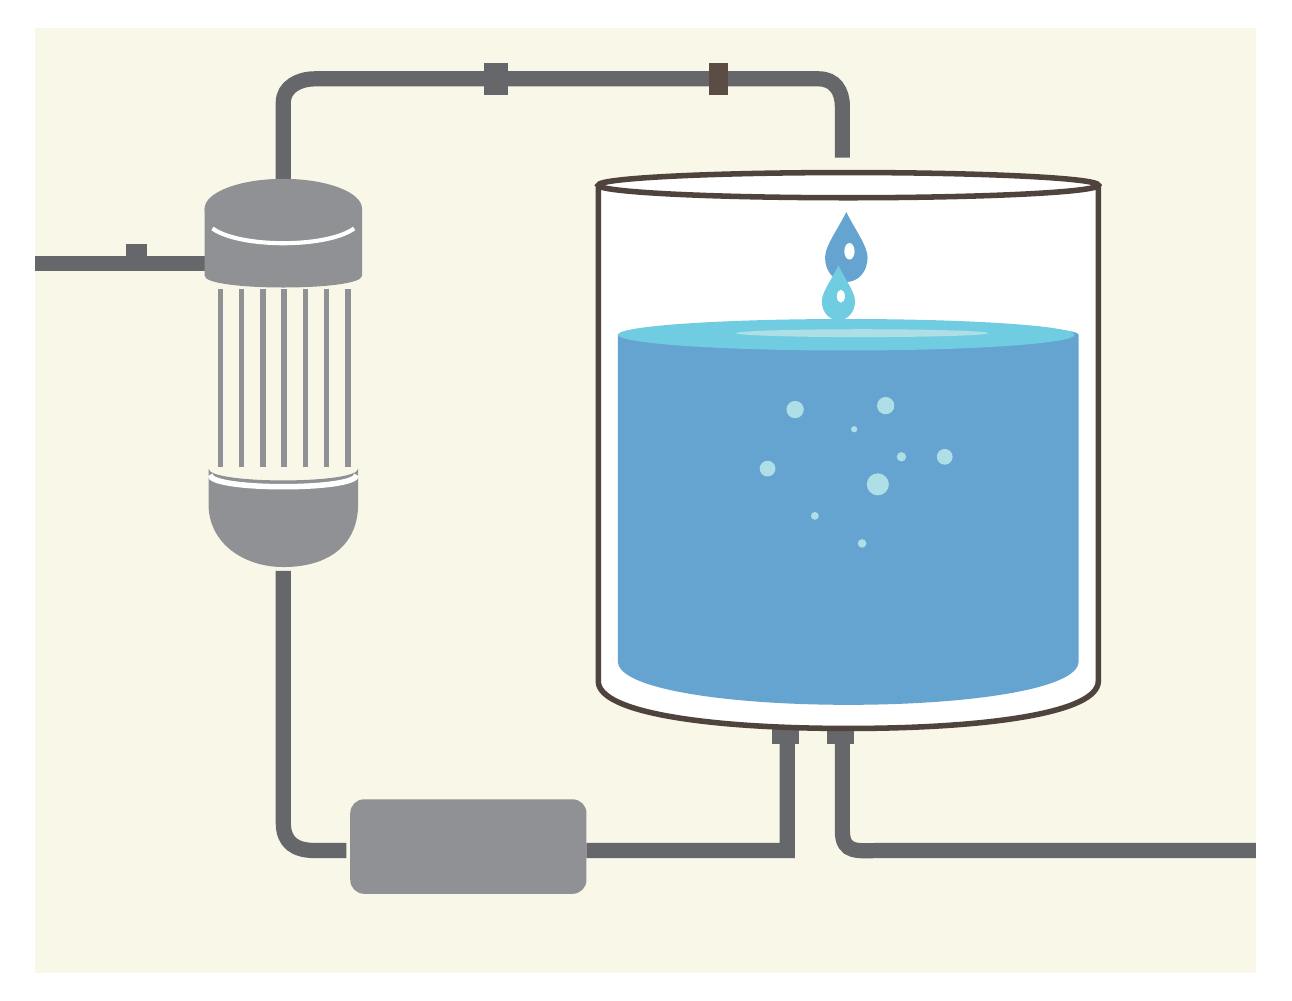
\begin{tikzpicture}
		\definecolor{papercream}{RGB}{249,247,232}
		\definecolor{paperstripe}{RGB}{222,220,203}
		\definecolor{pipegray}{RGB}{102,103,106}
		\definecolor{filtergray}{RGB}{143,145,148}
		\definecolor{filterdark}{RGB}{68,65,63}
		\definecolor{tankline}{RGB}{79,68,61}
		\definecolor{waterblue}{RGB}{101,164,208}
		\definecolor{waterlight}{RGB}{112,205,225}
		\definecolor{bubblecolor}{RGB}{174,222,230}
		\definecolor{couplingbrown}{RGB}{92,77,68}
		\path[fill=papercream] (0,2) rectangle (15.5,14);
		\draw[pipegray,line width=5.5pt]
			(3.15,12.05) -- (3.15,13.05)
			.. controls (3.15,13.25) and (3.35,13.35).. (3.55,13.35)
			-- (9.95,13.35)
			.. controls (10.15,13.35) and (10.25,13.20).. (10.25,13.00)
			-- (10.25,12.35);
		\fill[pipegray] (5.70,13.15) rectangle (6.00,13.55);
		\fill[couplingbrown] (8.55,13.15) rectangle (8.80,13.55);
		\draw[pipegray,line width=5.5pt] (0,11) -- (2.20,11);
		\fill[pipegray] (1.15,11) rectangle (1.42,11.25);
			(2.20,10.70) -- (4.10,10.70) -- (4.10,8.40)
			.. controls (4.10,8.20) and (2.20,8.20).. (2.20,8.40) -- cycle;
		\foreach \x in {2.35,2.62,2.89,3.16,3.43,3.70,3.97}{
			\draw[filtergray,line width=2pt] (\x,8.42) -- (\x,10.68);
		}
		\path[fill=filtergray]
			(2.2,8.4).. controls +(-90:0.2) and +(-90:0.2).. (4.1,8.4)
			-- (4.1,7.95).. controls +(-90:0.5) and +(0:0.6).. (3.15,7.15).. controls +(180:0.5) and +(-90:0.5).. (2.2,7.95) -- cycle;
		\draw[white,line width=2pt] (2.22,8.32).. controls +(-90:0.2) and +(-90:0.2).. (4.08,8.32);
		\path[fill=filtergray]
			(2.15,11.7).. controls +(90:0.2) and +(90:0.2).. (4.15,11.7)
			-- (4.15,10.85).. controls +(-90:0.2) and +(-90:0.2).. (2.15,10.85) -- cycle;
		\path[fill=filtergray]
			(3.15,11.70) ellipse [x radius=1.00,y radius=0.38];
		\draw[white,line width=1.5pt]
			(2.25,11.45).. controls (2.60,11.20) and (3.70,11.20).. (4.05,11.45);
		\draw[pipegray,line width=5.5pt]
			(3.15,7.10) -- (3.15,3.90)
			.. controls (3.15,3.65) and (3.30,3.55).. (3.55,3.55)
			-- (3.95,3.55)
			(7,3.55) -- (9.55,3.55) -- (9.55,5.40);
		\path[fill=filtergray,rounded corners=5pt] (4,4.2) rectangle +(3,-1.2);
		\draw[pipegray,line width=5.5pt]
			(10.25,5.35) -- (10.25,3.8).. controls +(-90:0.3) and +(180:0.3).. (10.75,3.55)-- (15.5,3.55);
		\fill[pipegray] (9.35,4.90) rectangle (9.70,5.35);
		\fill[pipegray] (10.05,4.90) rectangle (10.40,5.35);
		\draw[tankline,line width=2pt,fill=white]
			(7.15,12.00) -- (7.15,5.70)
			.. controls (7.15,5.30) and (8.55,5.10).. (10.325,5.10)
			.. controls (12.10,5.10) and (13.50,5.30).. (13.50,5.70)
			-- (13.50,12.00)
			(10.325,12.00) ellipse [x radius=3.175,y radius=0.16];
		\path[fill=waterblue]
			(7.40,10.10)
			.. controls (7.40,10.30) and (13.25,10.30).. (13.25,10.10)
			-- (13.25,5.95)
			.. controls (13.25,5.60) and (11.85,5.40).. (10.325,5.40)
			.. controls (8.80,5.40) and (7.40,5.60).. (7.40,5.95) -- cycle;
		\path[fill=waterlight]
			(10.3,10.10) ellipse [x radius=2.9,y radius=0.2];
		\path[fill=bubblecolor] (10.5,10.12) ellipse [x radius=1.60,y radius=0.05];
		\foreach \x/\y/\r in {
			9.65/9.15/0.11,
			10.80/9.20/0.11,
			11.55/8.55/0.10,
			10.40/8.90/0.04,
			9.30/8.40/0.10,
			11.00/8.55/0.06,
			10.70/8.20/0.14,
			9.90/7.80/0.05,
			10.50/7.45/0.055
			}{
			\path[fill=bubblecolor] (\x,\y) circle (\r);
		}
		\newcommand{\waterdrop}[4]{%
		\begin{scope}[shift={(#1,#2)},scale=#3]
			\path[fill=#4]
				(0,0.46)
				.. controls (-0.10,0.25) and (-0.27,0.03).. (-0.27,-0.12)
				.. controls (-0.27,-0.30) and (-0.15,-0.43).. (0,-0.43)
				.. controls (0.15,-0.43) and (0.27,-0.30).. (0.27,-0.12)
				.. controls (0.27,0.03) and (0.10,0.25).. (0,0.46)
				-- cycle;
			\path[fill=white]
				(0.04,-0.04) ellipse [x radius=0.065,y radius=0.105];
		\end{scope}%
		}
		\waterdrop{10.3}{11.2}{1.0}{waterblue}
		\waterdrop{10.2}{10.62}{0.78}{waterlight}
	\end{tikzpicture}
	}}

	\begin{loigiai}
		Ta có
		\[h'(t)=3at^2+bt\Rightarrow h(t)=\displaystyle\int\left(3at^2+bt\right)\mathrm{\,d}t=at^3+\dfrac{1}{2}bt^2+C.\]
		Vì ban đầu bể không có nước ($h(0)=0$) nên $C=0$.\\
		Do đó $h(t)=at^3+\dfrac{1}{2}bt^2.$\\
		Ta có
		\begin{itemize}
			\item $h(5)=150\Rightarrow 125a+\dfrac{25}{2}b=150$.
			\item $h(10)=1\,100\Rightarrow 1\,000a+50b=1\,100$.
		\end{itemize}
		Do đó
		$\heva{&125a+\dfrac{25}{2}b=150\\
		&1\,000a+50b=1\,100}\Rightarrow\heva{&a=1\\&b=2.}$\\
		Suy ra $h(t)=t^3+t^2$. \\
		Vậy thể tích nước của bể sau $20$ giây là
		\[h(20)=20^3+20^2=8\,000+400=8\,400~\mathrm{m}^3.\]
	\end{loigiai}
\end{baitap}

%%%=================SLIDE THONG KE=================%%%
\thongke

\end{document}